%% LaTeX-Beamer template for KIT design
%% by Erik Burger, Christian Hammer
%% title picture by Klaus Krogmann
%%
%% version 2.1
%%
%% mostly compatible to KIT corporate design v2.0
%% http://intranet.kit.edu/gestaltungsrichtlinien.php
%%
%% Problems, bugs and comments to
%% burger@kit.edu

\documentclass[18pt]{beamer}
\usepackage[utf8]{inputenc}
\usepackage{algpseudocode}
\usepackage{listings}
\usepackage{amsfonts} 
\usepackage{mathtools} 
\usepackage{alltt}
%% SLIDE FORMAT

% use 'beamerthemekit' for standard 4:3 ratio
% for widescreen slides (16:9), use 'beamerthemekitwide'

\usepackage{templates/beamerthemekit}
% \usepackage{templates/beamerthemekitwide}

%% TITLE PICTURE

% if a custom picture is to be used on the title page, copy it into the 'logos'
% directory, in the line below, replace 'mypicture' with the 
% filename (without extension) and uncomment the following line
% (picture proportions: 63 : 20 for standard, 169 : 40 for wide
% *.eps format if you use latex+dvips+ps2pdf, 
% *.jpg/*.png/*.pdf if you use pdflatex)

%\TitleImage[width=\titleimagewd]{pics/title}
%\titleimage{}

%% TITLE LOGO

% for a custom logo on the front page, copy your file into the 'logos'
% directory, insert the filename in the line below and uncomment it

%\titlelogo{mylogo}

% (*.eps format if you use latex+dvips+ps2pdf,
% *.jpg/*.png/*.pdf if you use pdflatex)

%% TikZ INTEGRATION

% use these packages for PCM symbols and UML classes
% \usepackage{templates/tikzkit}
% \usepackage{templates/tikzuml}
\usepackage{listings}
\usepackage{color}

\definecolor{dkgreen}{rgb}{0,0.6,0}
\definecolor{gray}{rgb}{0.5,0.5,0.5}
\definecolor{mauve}{rgb}{0.58,0,0.82}

\lstset{frame=tb,
  language=Java,
  aboveskip=3mm,
  belowskip=3mm,
  showstringspaces=false,
  columns=flexible,
  basicstyle={\small\ttfamily},
  numbers=none,
  numberstyle=\tiny\color{gray},
  keywordstyle=\color{blue},
  commentstyle=\color{dkgreen},
  stringstyle=\color{mauve},
  breaklines=true,
  breakatwhitespace=true
  tabsize=3
}


\setbeamertemplate{enumerate items}[circle]
% the presentation starts here

\title[Algo Tutorium Nr.2]{Algorithmen I - Sommersemester 2014}
\subtitle{Tutorium Nr. 2}
\author{Tobias Hornberger}

\institute{Institut für Theoretische Informatik}

\begin{document}

% change the following line to "ngerman" for German style date and logos
\selectlanguage{ngerman}

%title page
\begin{frame}
\titlepage
\end{frame}

%table of contents
%~ \begin{frame}[allowframebreaks]{Übersicht}
%~ \tableofcontents
%~ \end{frame}


\section{Organisatorisches}
\subsection{Übungsblätter}
\begin{frame}
	\begin{center}
 			\huge{Rückgabe der Übungsblätter} \\
 			\parskip 36pt
 			\normalsize{$\rightarrow$ Bei Rückfragen bitte am Ende des Tutoriums vorkommen}
 		\end{center}
 	\end{frame}
 
 \subsection{Email-Liste}
 
 	\begin{frame}{Email-Liste}
 		Nach dem Email-Desaster: \\
 		\parskip 20pt
 		\begin{block}{Kommunikation}
 			\begin{itemize}
 				\item Bitte Email auf dem Blatt eintragen
 				\item Nach dem Tutorium schauen ob meine Email angekommen ist
 			\end{itemize}
 		\end{block}
 	\end{frame}

\section{Rekurrenzen}
\subsection{Aufgabe}
\begin{frame}{Rekurrenz Beispiel}
	\begin{center}
		$ T(n)=\left\{\begin{array}{cr} 1, & \mbox{falls } n = 1\\ 2 T(\lfloor n / 2 \rfloor) + n, & \mbox{falls } n \geq 2 \end{array}\right. $

		\parskip 14pt
		$n \in 2 ^{m} $ für $ m \in \mathbb{N} _{0} $

	\end{center}
	\begin{block}{Vorgehen}
		\begin{enumerate}
			\item Lösung raten...
			\item Beweisen, dass die Lösung stimmt
		\end{enumerate}
	\end{block}
\end{frame}

\begin{frame}{Substitutieren und Einsetzen}
	Umformung:
	\begin{align*}
		T(n) &= 2 T(\lfloor n / 2 \rfloor) + n \text{ mit } T(1) = 1\\
		T(2^m) &= 2* T(2^{m - 1}) + 2^m \text{ mit } T(1) = 1\\
		S(m) &= 2 * S(m-1) + 2^m \text{ mit } S(0) = 1
	\end{align*}
	Ausrechnen der ersten Werte:
	\begin{align*}
		S(0) &= T(2^0) = T(1)  = 1\\
		S(1) &= T(2^1) = T(2)  = 2 * 1 + 2 = 4\\
		S(2) &= T(2^2) = T(4)  = 2 * (2 * 1 + 2) + 4 = 12\\
		S(3) &= T(2^3) = T(8)  = 2 * (2 * (2 * 1 + 2) + 4 ) + 8 = 32\\
		S(4) &= T(2^4) = T(16) = 2 * ( 2 * (2 * (2 * 1 + 2) + 4 ) + 8 ) + 16 = 70
	\end{align*}
\end{frame}

\subsection{Lösung}
\begin{frame}{Lösung raten}
	\[
		S(m) = 2 * S(m-1) + 2^m \text{ mit } S(0) = 1
	\]
	\begin{align*}
		S(0) &= 1 = 2^0\\
		S(1) &= 2 * 1 + 2 = 2^1 + 2^1 = 2^2\\
		S(2) &= 2 * (2 * 1 + 2) + 4 = 2^3 + 2^2\\
		S(3) &= 2 * (2 * (2 * 1 + 2) + 4 ) + 8 = 2^4 + 2 * 2^3\\
		S(4) &= 2 * ( 2 * (2 * (2 * 1 + 2) + 4 ) + 8 ) + 16 = 2^5 + 3 * 2^4
	\end{align*}

	Durch scharfes Hinsehen erkennen wir eine mögliche Lösung:

	$$S(m) = 2^{m+1} + (m-1) * 2^{m}$$

	Beweis der Lösung durch vollständige Induktion.
\end{frame}

\subsection{Korrektheitsbeweis}
\begin{frame}{Beweis durch vollständige Induktion}
	\textbf{IA:} $S(0) = T(2^0) = T(1) = 1$ \\
	\textbf{IV:} $S(m) = 2^{m+1} + (m - 1)*2^{m}$\\
	\textbf{IS:} m $\rightarrow$ $m+1$
	\begin{align}
		S(m+1)& = 2 * S(m) + 2^{m+1} \\
		& = 2 * ( 2^{m+1} + (m-1) * 2^m) + 2^{m+1} \\
		& = 2^{m+2} + (m-1) * 2^{m+1} + 2^{m+1} \\
		& = 2^{m+2} + m * 2^{m+1}
	\end{align}
	\ \\
	Zurück nach T(n) rechnen für Finale Lösung: \\
	$T(n) = S(\log _2 n) = 2^{\log _2 n + 1} * (\log _2 n - 1) * 2 ^{\log _2 n}$
\end{frame}

\section{Datenstrukturen}
\subsection{Listen}
\begin{frame}[fragile]
	\frametitle{Listen}
	\begin{columns}[t]
		\column{.5\textwidth}
\begin{verbatim}
Class Item of Element:
    e : Element
    next : Pointer to Item
    prev : Pointer to Item
\end{verbatim}
		\column{.5\textwidth}
\begin{alltt}
Class List of Element:
    h = Item(\(\bot\),
      h,
      h)
\end{alltt}
	\end{columns}
	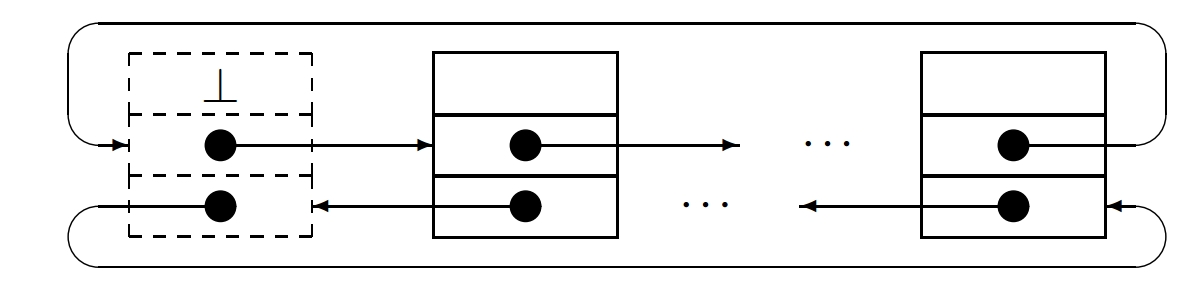
\includegraphics[width=\textwidth]{logos/list}
\end{frame}

\begin{frame}
	\frametitle{Laufzeiten für Operationen auf Listen}
	\begin{itemize}
		\item Einfügen am Anfang \only<2->{\textbf{$\mathcal{O}(1)$}}
		\item Einfügen am Ende \only<3->{\textbf{$\mathcal{O}(1)$}}
		\item Element finden \only<4->{\textbf{$\mathcal{O}(n)$}}
		\item Element entfernen (mit Verweis auf Element) \only<5->{\textbf{$\mathcal{O}(1)$}}
		\item Zusammenfügen zweier Listen \only<6->{\textbf{$\mathcal{O}(1)$}}
		\item Zugriff auf das $k$-te Element \only<7->{\textbf{$\mathcal{O}(n)$}}
		\item Aufteilen einer Liste in zwei (mit Verweis auf Stelle) \only<8->{\textbf{$\mathcal{O}(1)$}}
		\item Länge der Liste bestimmen \only<9->{\textbf{$\mathcal{O}(n)$}}
	\end{itemize}
\end{frame}

\subsection{Aufgaben zu Listen}
\begin{frame}
	\frametitle{Aufgabe zu Listen}
	Implementiert folgende Operationen für eine doppelt verkettete, \emph{sortierte} Liste in Pseudocode:

	\begin{enumerate}
		\item \emph{insert(e)} (Einfügen des Elements $e$ an die richtige Stelle)
		\item \emph{findFirst(e)} (Erstes Vorkommen von $e$ in der Liste)
		\item \emph{remove(e)} (Entfernen des Elements $e$ aus der Liste)
	\end{enumerate}
\end{frame}

\section{Amortisierte Analyse}
\begin{frame}
	\frametitle{Amortisierte Analyse}
	\begin{itemize}
		\item gemittelter Aufwand für eine Sequenz von Operationen im Worst-case
		\item Kosten einer Operation gering, auch wenn eine einzelne Operation kostspielig ist
		\item keine Einbeziehung von Wahrscheinlichkeiten
		\item Beispiel: unbounded Arrays 
	\end{itemize}
\end{frame}

\begin{frame}
	\frametitle{Konto-Methode}
	für jede Operation:
	\begin{itemize}
		\item $\hat{c}_i$ \textbf{amortisierte Kosten}
		\item $c_i$ \textbf{tatsächliche Kosten}
		\item $\hat{c}_i \geq c_i  \Rightarrow $  Guthaben einzahlen
		\item $\hat{c}_i \leq c_i  \Rightarrow $  Guthaben abheben
		\item Konto darf \textbf{nie} negativ werden
		\begin{itemize}
			\item $ \forall n \in \mathbb{N} : c + \sum_{i=1} ^n \hat{c}_i \geq \sum_{i=1} ^n c_i$
		\end{itemize}

	\end{itemize}

\end{frame}

\begin{frame}
	\frametitle{Beispiel: Unbounded Arrays}

	\begin{itemize}
		\item falls ein Feld mit \textit{n} Elementen durch \textbf{reallocate} verkleinert oder vergrößert wird,
		 müssen \textit{n} Elemente kopiert werden $\Rightarrow$ \textit{n} Tokens müssen vorhanden sein
		\item amortisierte Kosten:
		\begin{itemize}
			\item \textbf{push}: 3 Tokens
			\begin{itemize}
				\item 1 Token: Einfügen des Elements
				\item 2 Tokens: Konto
			\end{itemize}
			\item \textbf{pop}: 2 Tokens
			\begin{itemize}
				\item 1 Token: Löschen des Elements
				\item 1 Token: Konto
			\end{itemize}
		\end{itemize}
	\end{itemize}

\end{frame}

\begin{frame}
	\frametitle{Beispiel: Unbounded Arrays}
	\begin{itemize}
		\item Anfangszustand nach \textbf{reallocate}:
		\begin{itemize}
			\item \textit{n} Elemente, kein Guthaben vorhanden \\ \ \\
		\end{itemize}


		\item Sequenz von \textbf{push}-Operationen:
		\begin{itemize}
			\item \textbf{reallocate} wird nach \textit{n} \textbf{push}-Operationen aufgerufen
			\item Guthaben: 2\textit{n} Tokens
			\item \textbf{reallocate}-Aufruf: 2\textit{n} Elemente werden kopiert $\rightarrow$ genug Tokens \\ \ \\
		\end{itemize} 

		\item Sequenz von \textbf{pop}-Operationen:
		\begin{itemize}
			\item \textbf{reallocate} wird nach \textit{$\frac{n}{2}$} \textbf{pop}-Operationen aufgerufen
			\item Guthaben: \textit{$\frac{n}{2}$} Tokens
			\item \textbf{reallocate}-Aufruf: \textit{$\frac{n}{2}$} Elemente werden kopiert $\rightarrow$ genug Tokens \\ \ \\
		\end{itemize} 

	\end{itemize}
\end{frame}

\section{Kreativaufgabe}

\subsection{Aufgabenteil a)}
\begin{frame}
	\frametitle{Kreativaufgabe (a)}
	Entwickelt eine Datenstruktur mit folgenden Eigenschaften:

	\begin{itemize}
		\item \emph{pushBack} und \emph{popBack} in $\mathcal{O}(1)$
		\item Zugriff auf das $k$-te Element in $\mathcal{O}(\log{n})$
	\end{itemize}

	Jeweils für Worst-Case und nicht amortisiert.
	Speicherallokation ist dabei immer in $\mathcal{O}(1)$.
\end{frame}

\subsection{Aufgabenteil b)}

\begin{frame}
	\frametitle{Kreativaufgabe (b)}
	Jetzt umgekehrt:

	\begin{itemize}
		\item \emph{pushBack} und \emph{popBack} in $\mathcal{O}(\log{n})$
		\item Zugriff auf das $k$-te Element in $\mathcal{O}(1)$
	\end{itemize}

	Jeweils für Worst-Case und nicht amortisiert.
	Speicherallokation ist dabei immer in $\mathcal{O}(1)$.
\end{frame}


\end{document}
